%%%%%%%%%%%%%%%%%%%%%%%%%%%%%%%%%%%%%%%%%%%%%%%%%%%%%%%%%%%%%%%%%%%%%%%%%%%%%%%%%%%%%%%%%%%%%%%%%%%%%%%%%%%%%%%%%%%%%%
\chapter{Compare time integration methods}
%%%%%%%%%%%%%%%%%%%%%%%%%%%%%%%%%%%%%%%%%%%%%%%%%%%%%%%%%%%%%%%%%%%%%%%%%%%%%%%%%%%%%%%%%%%%%%%%%%%%%%%%%%%%%%%%%%%%%%
%!!!!!!!!!!!!!!!!!!!!!!!!Endre $y$( $u$ eller $U$) til noe annet!!!!!!!!!!!!!!!!!!!!\\
%!!!!!!!!!!!!!!!!!!!!!!!!Oppdater iterasjonsskjema for midpoint rule!!!!!!!!!!!!!!!!!!!!\\
!!!!!!!!!!!!!!!!!!!!!!!!Legg til errorplott!!!!!!!!!!!!!!!!!!\\
!!!!!!!!!!!!!!!!!!!!!!!!Se hvordan energien øker ved større tidslengde!!!!!!!!!!!\\
!!!!!!!!!!!!!!!!!!!!!!!!!!!!!Dimensjoner på $I$-er i integrasjonsmetodene?!!!!!!!!!!!!!!!!!!!!\\
!!!!!!!!!!!!!!!!!!!!!!!!!!!!!!!!Teste på problemer med ikke konstant energi!!!!!!!!!!!!!!!!!!!!!!\\
This section will be concerned with comparing the integrators. How well they estimate the error and energy will be the primary concern.\\

The relevant integrators are trapezoidal rule, forward euler, and midpoint rule. The definition, and the iteration scheme, of the different methods are given in the table below. 

\begin{table}
\begin{tabular}{l l}
	Trapezoidal rule \cite{trapezoidal} & $U_{i+1} = U_{i}+h_t g \Big( \frac{1}{2}(t_i+t_{i+1}),\frac{1}{2}(U_i+U_{i+1}) \Big)$
	\\ & $U_{i+1} = (I- \frac{A h_t}{2}) ^{-1} \Big(  U_i + \frac{h_t}{2} \big( A U_i+(F_{i+1}+F_i) \big)  \Big) $\\
	Forward Euler \cite{forwardeuler} & $ U_{i+1} = U_i + h_t g ( t_i, U_i ) $ \\ & $ U_{i+1} = U_i + h_t \big( A U_i + F_i \big) $ \\
	Midpoint rule \cite{midpoint} & $U_{i+1} = U_i + h_t + g \Big(  t_{i+\frac{1}{2}} , \frac{1}{2}(U_i + U_{i+1})    \Big) $ \\ & 
	$U_{i+\frac{1}{2}} = U_i + \frac{h_t}{2} ( A U_i + F_i )$ \\ &
    $U_{i+1} = (I-\frac{A h_t}{2}) ^{-1} (U_{i+\frac{1}{2}} + \frac{h_t}{2} F_{i+ \frac{1}{2}})$
\end{tabular}
\label{tab:intmet}
\caption{ Proposed methods for integrating in time. Note that since the midpoint rule uses $F_{i+\frac{1}{2}}$ and because of the restart, we need to save twice as many points in time for midpoint rule, as for the others !!!!!!Skriv noe om hva dette betyr!!!. Er denne tabellen fin nok?}
\end{table}

Convergence of the different methods are shown in figure \ref{fig:intconv}

\begin{figure}[H]
        \centering
        \begin{subfigure}[b]{0.30\textwidth}
                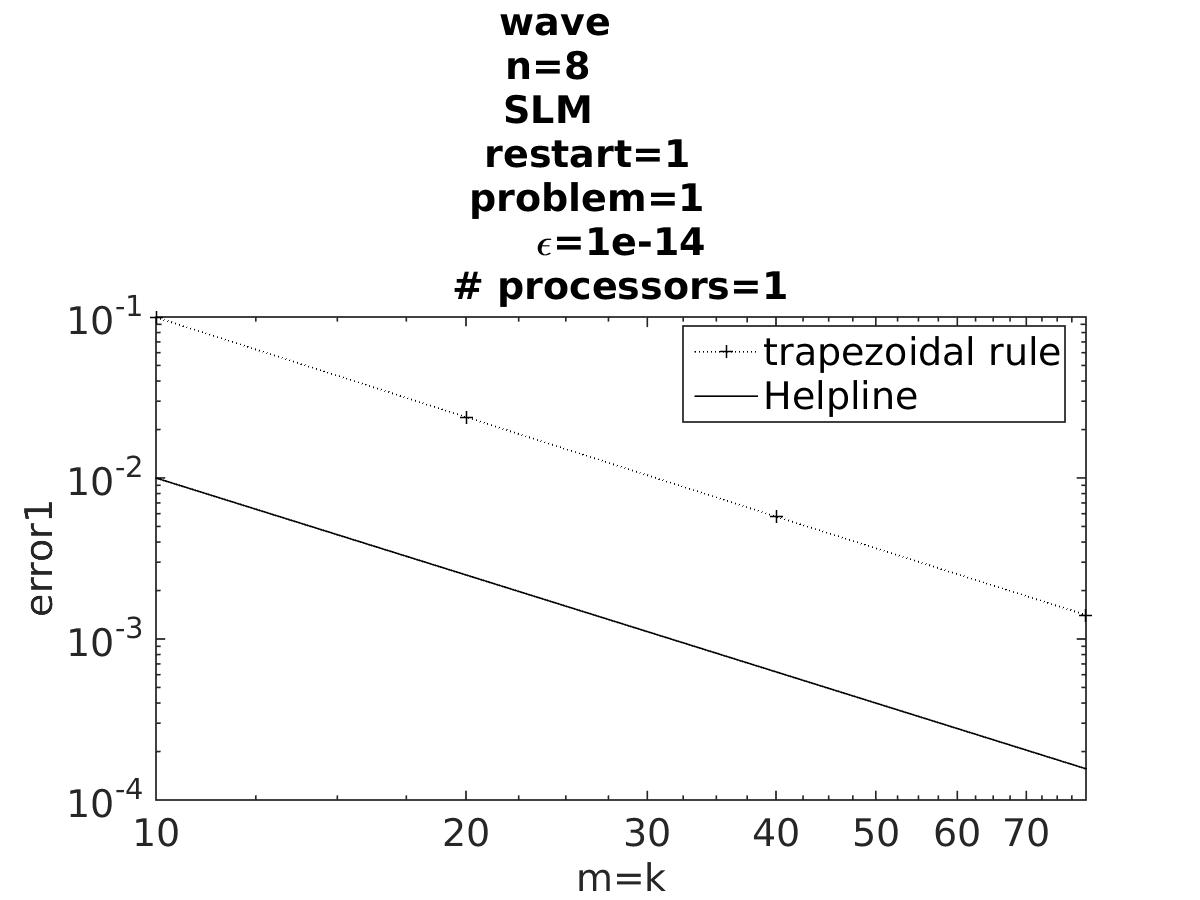
\includegraphics[width=\textwidth]{../MATLAB/fig/intconvtrap.jpg}
                %\includegraphics[width=\textwidth]{test}
                \caption{ Help line decreases with $m^2$. }
                \label{fig:intconvtrap}
        \end{subfigure}%
        ~
        \begin{subfigure}[b]{0.30\textwidth}
                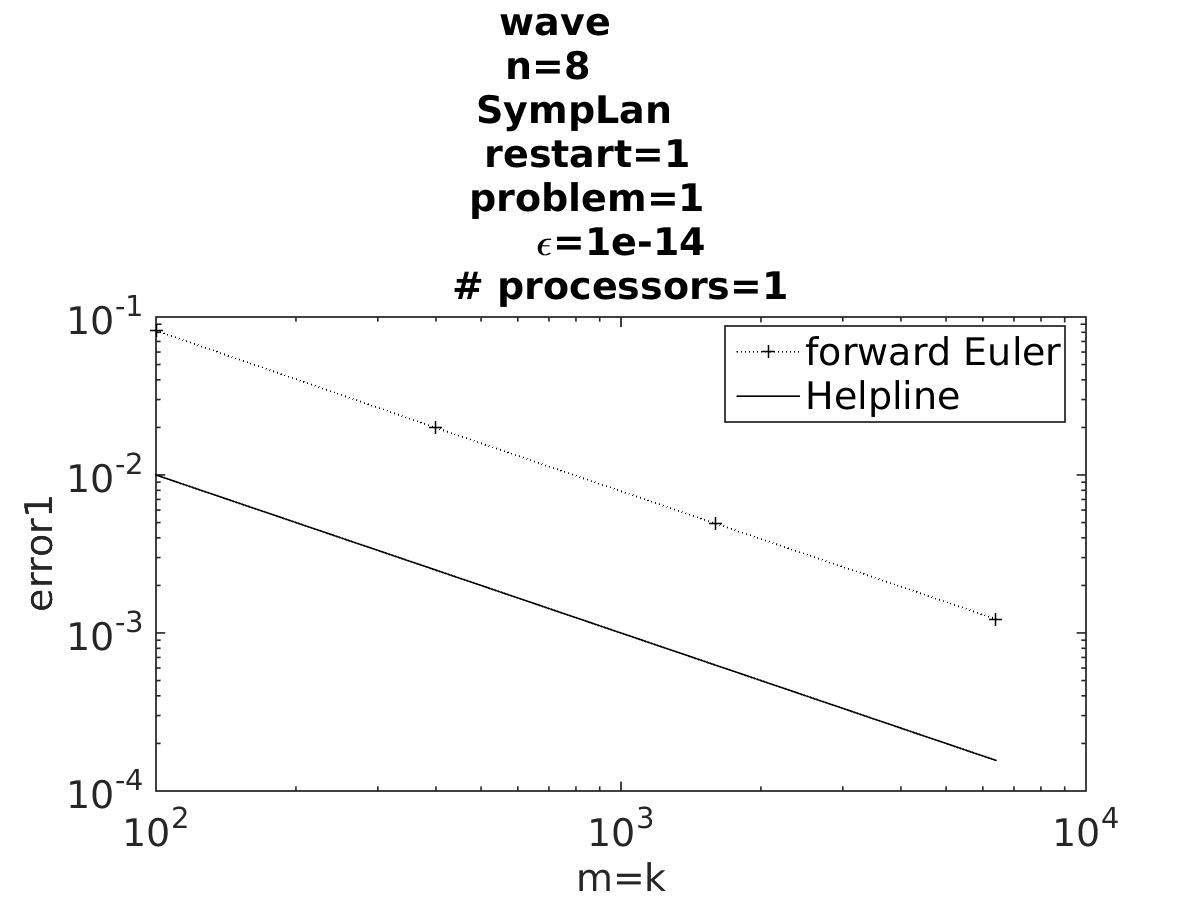
\includegraphics[width=\textwidth]{../MATLAB/fig/intconveul.jpg}
                %\includegraphics[width=\textwidth]{test}
                \caption{ Help line decreases with $m$. }
                \label{fig:intconveul}
        \end{subfigure}
        \begin{subfigure}[b]{0.30\textwidth}
                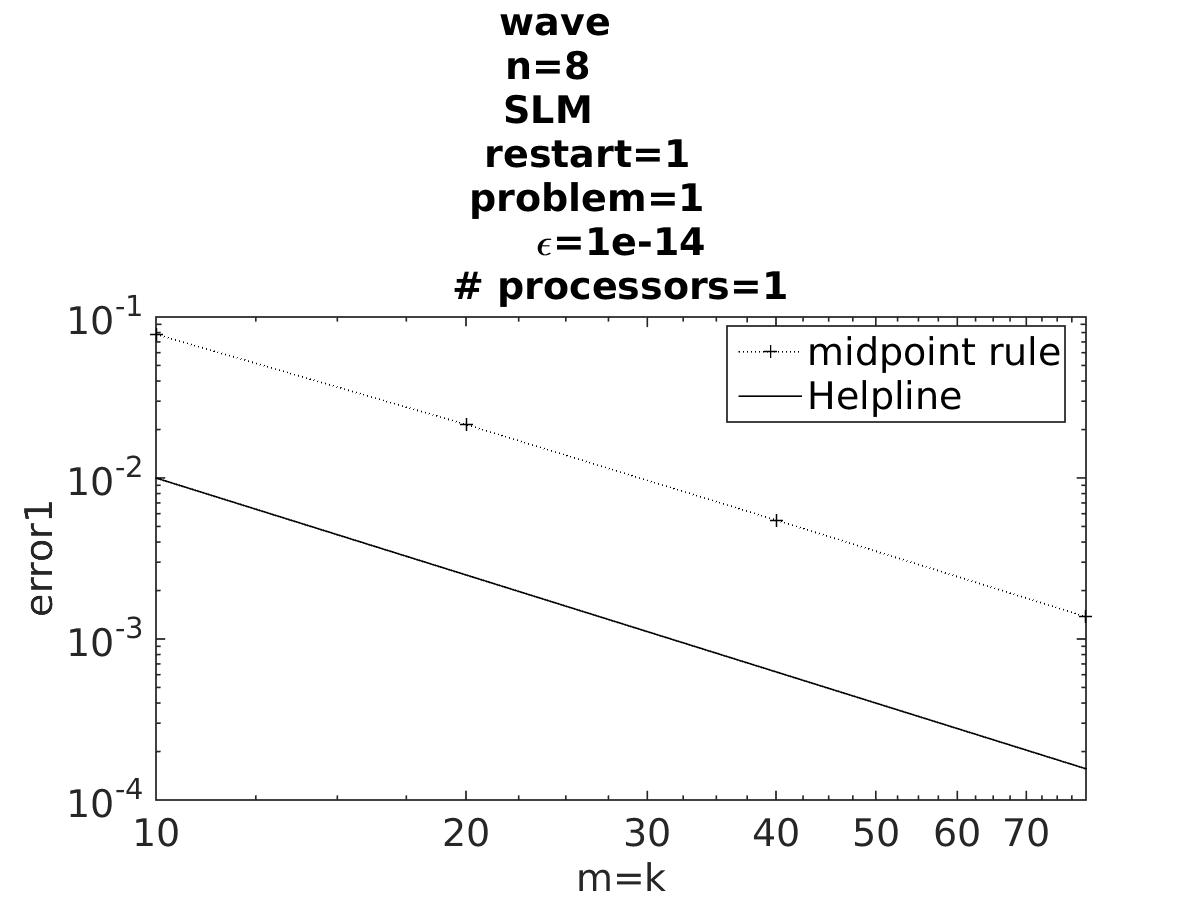
\includegraphics[width=\textwidth]{../MATLAB/fig/intconvmid.jpg}
                %\includegraphics[width=\textwidth]{test}
                \caption{ Help line decreases with $m^2$. }
                \label{fig:intconvmid}
        \end{subfigure}
        
        
        \caption{Figure of the convergence for the different integration methods. All methods converge with the expected rate. }
        \label{fig:intconv}
\end{figure}


\begin{figure}[H]
        \centering
        \begin{subfigure}[b]{0.30\textwidth}
                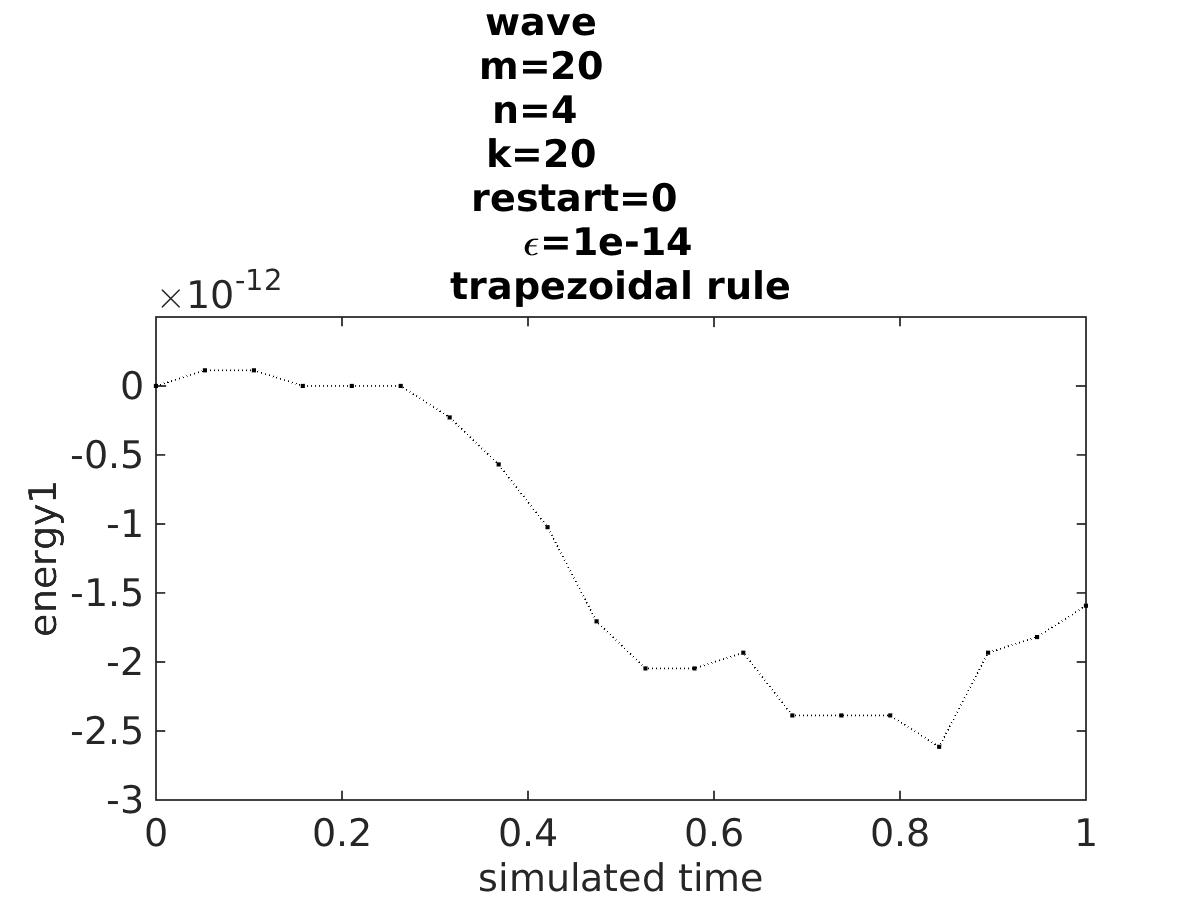
\includegraphics[width=\textwidth]{../MATLAB/fig/energyovertimetrapezoidal.jpg}
                \caption{  }
                \label{fig:energyovertimetrapezoidal}
        \end{subfigure}%
        ~
        \begin{subfigure}[b]{0.30\textwidth}
                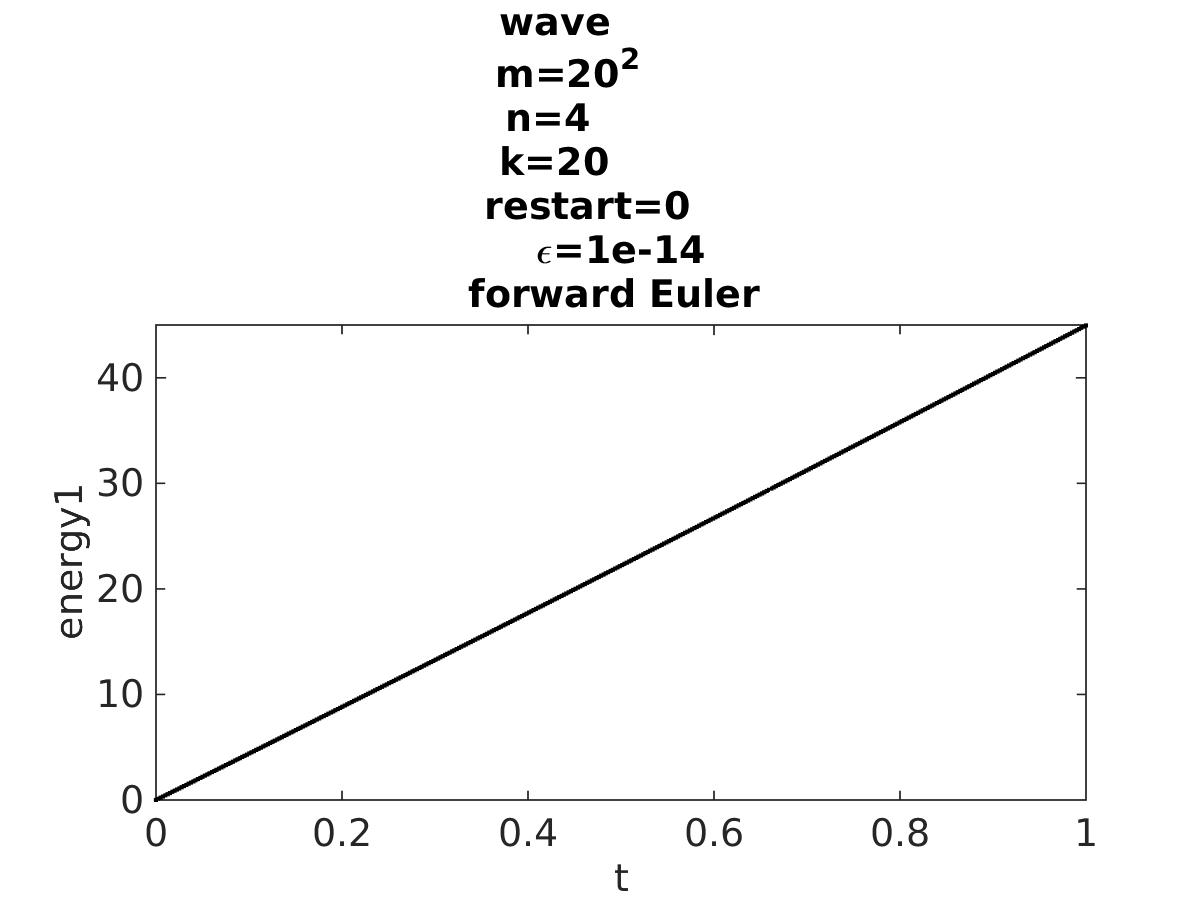
\includegraphics[width=\textwidth]{../MATLAB/fig/energyovertimeeuler.jpg}
                \caption{  }
                \label{fig:energyovertimeeuler}
        \end{subfigure}
        \begin{subfigure}[b]{0.30\textwidth}
                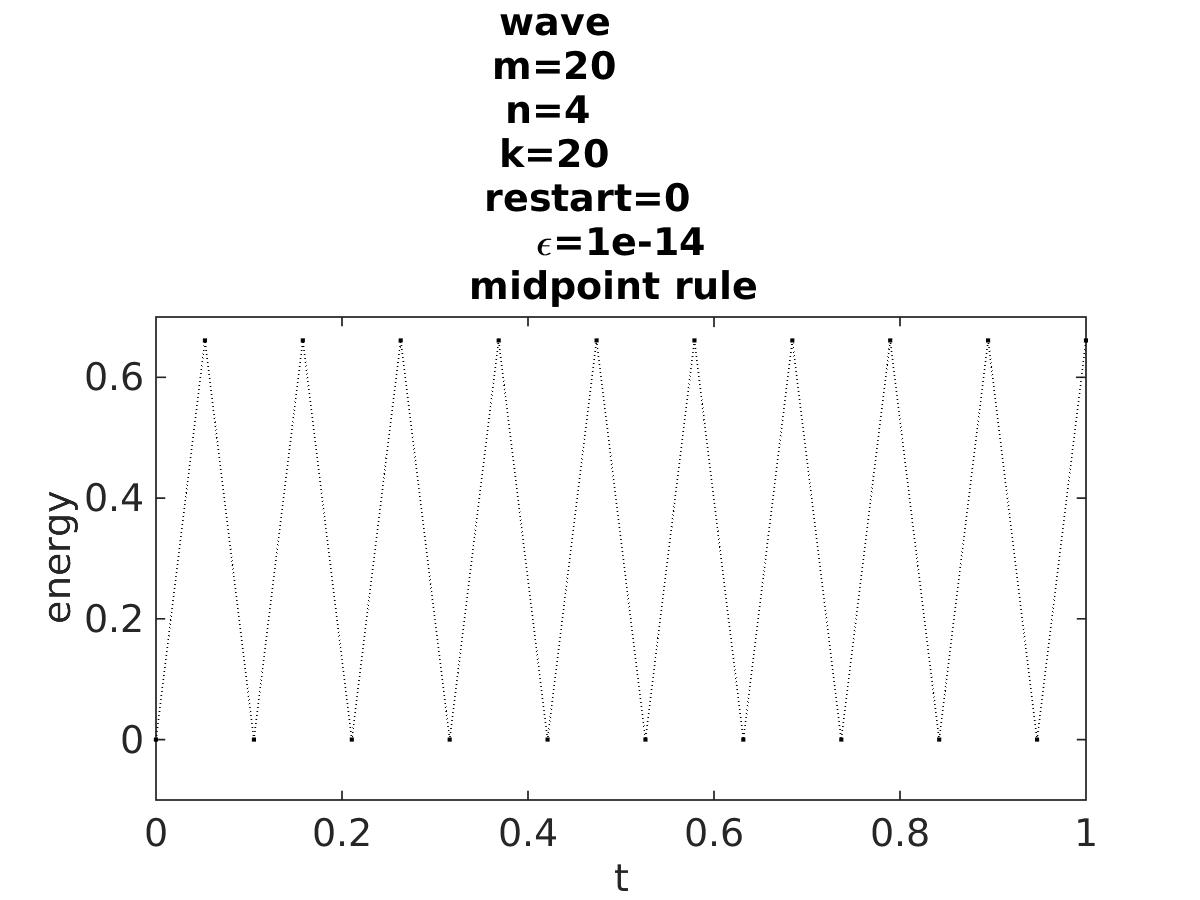
\includegraphics[width=\textwidth]{../MATLAB/fig/energyovertimemidpoint.jpg}
                \caption{  }
                \label{fig:energyovertimemidpoint}
        \end{subfigure}
        
        \begin{subfigure}[b]{0.30\textwidth}
                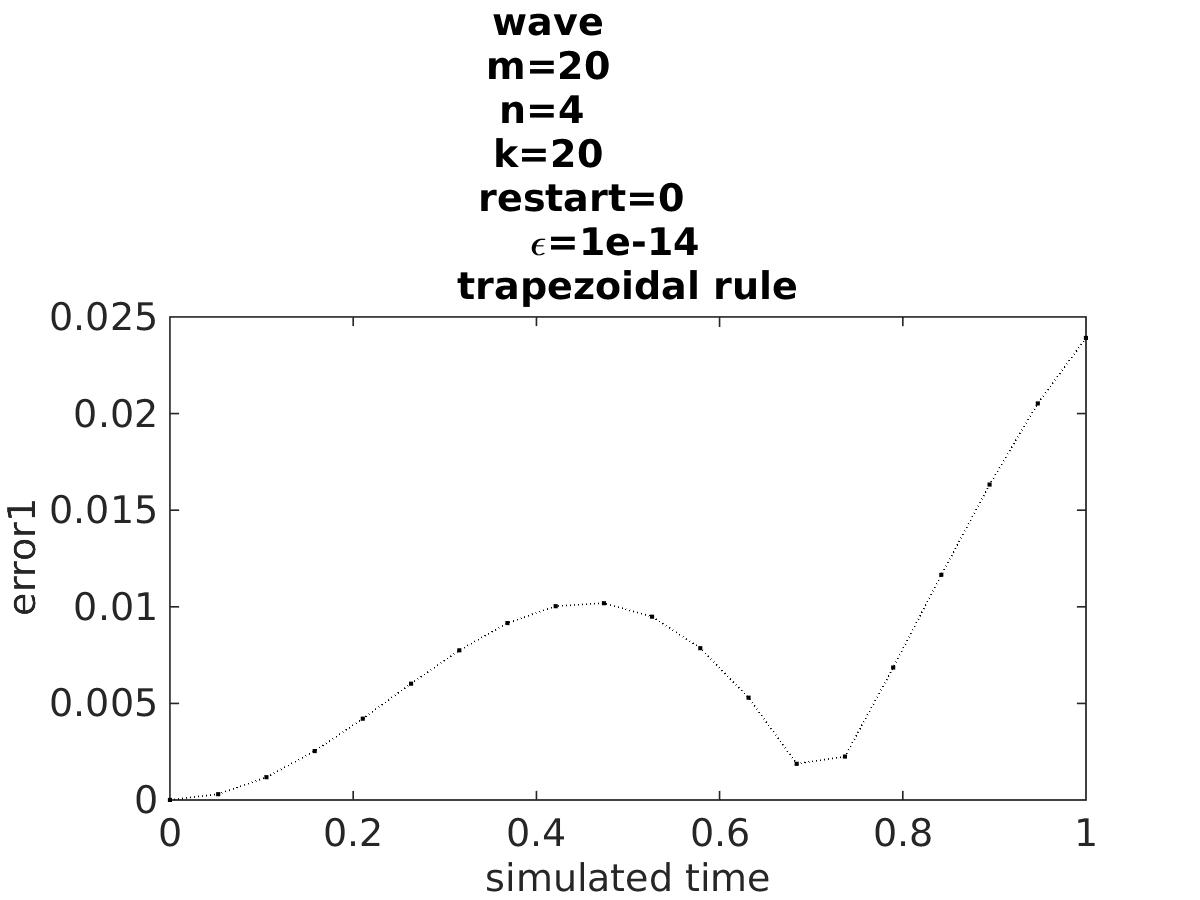
\includegraphics[width=\textwidth]{../MATLAB/fig/errorovertimetrapezoidal.jpg}
                \caption{  }
                \label{fig:errorovertimetrapezoidal}
        \end{subfigure}%
        ~
        \begin{subfigure}[b]{0.30\textwidth}
                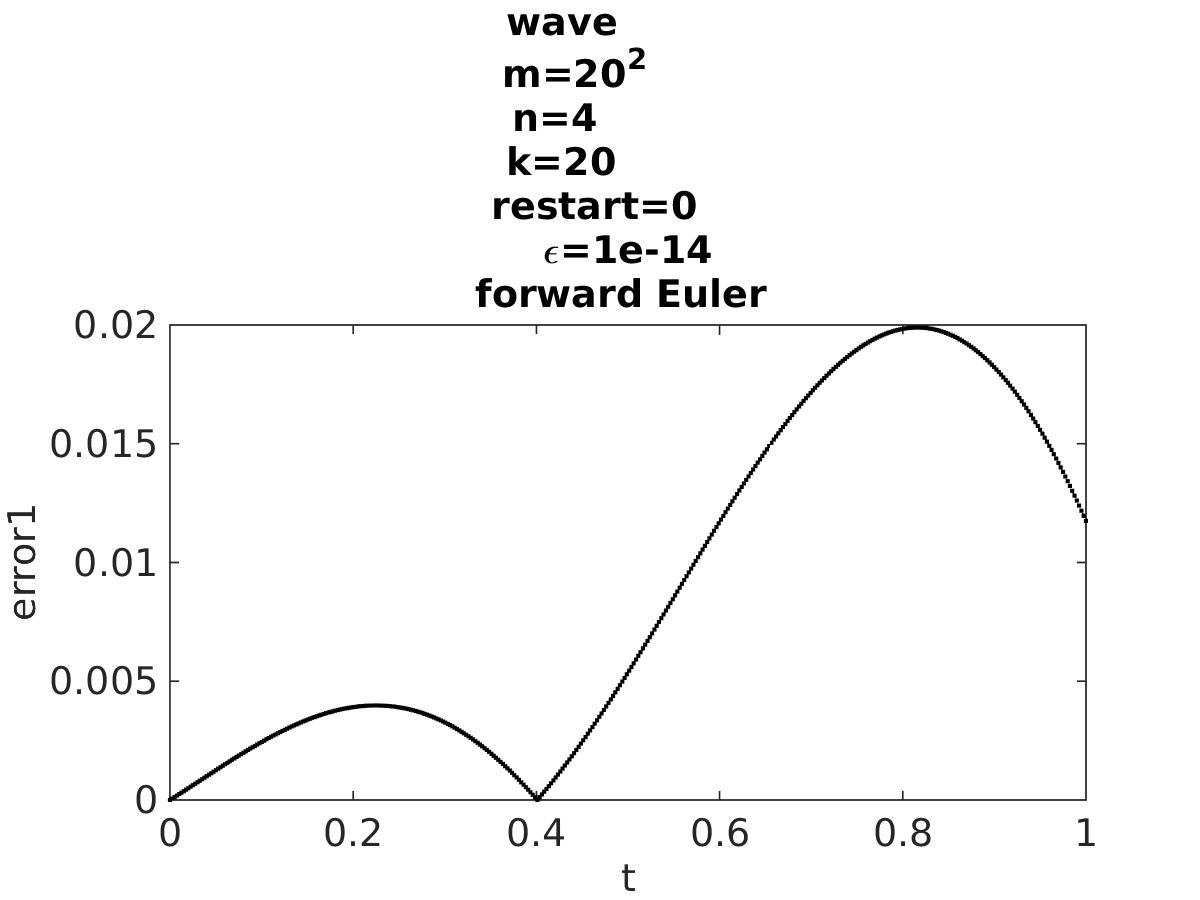
\includegraphics[width=\textwidth]{../MATLAB/fig/errorovertimeeuler.jpg}
                \caption{  }
                \label{fig:errorovertimeeuler}
        \end{subfigure}
        \begin{subfigure}[b]{0.30\textwidth}
                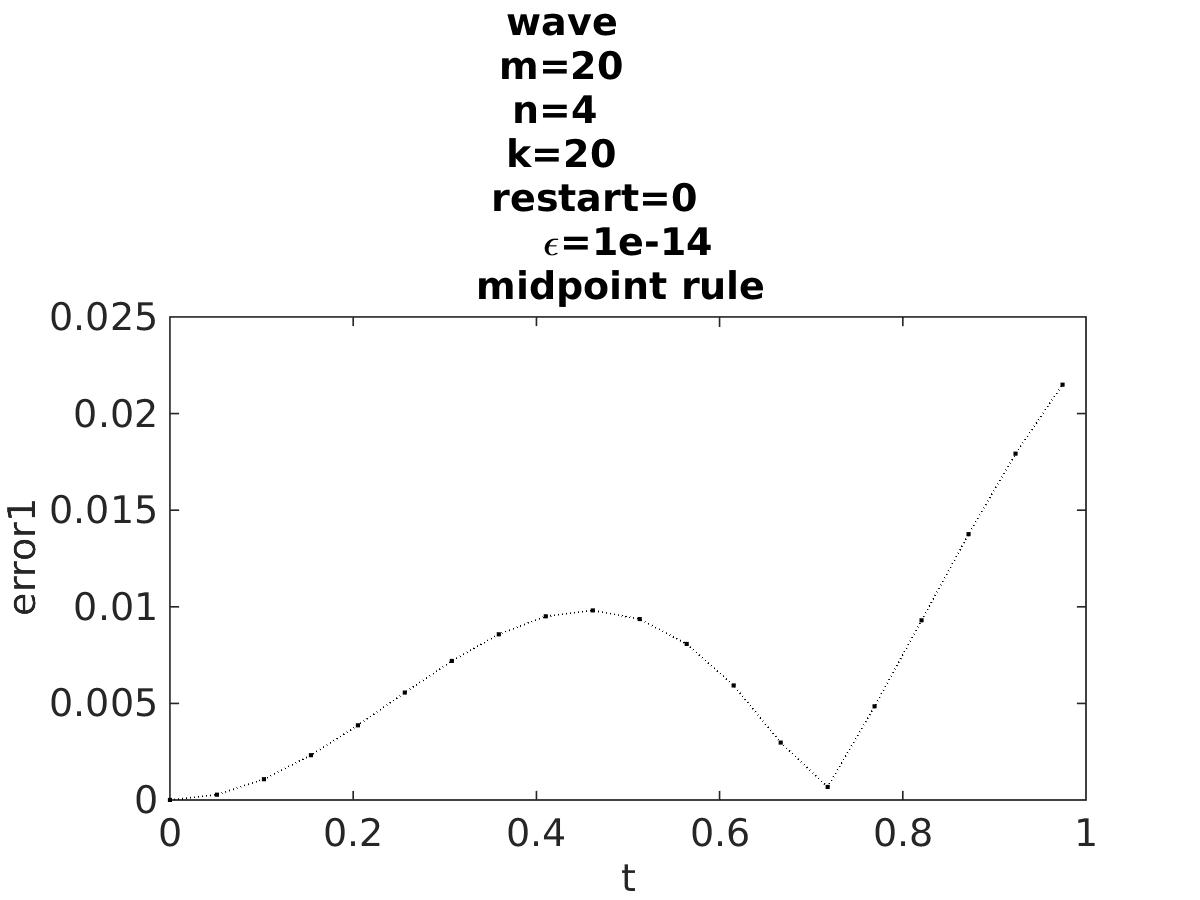
\includegraphics[width=\textwidth]{../MATLAB/fig/errorovertimemidpoint.jpg}
                \caption{  }
                \label{fig:errorovertimemidpoint}
        \end{subfigure}
        \caption{Figure of the difference in energy at a point in time. It is clear that only trapezoidal rule gives a suitable approximation of the error. Forward euler has an linearly increasing energy, while the midpoint rule gives periodic energy.}
        \label{fig:error}
\end{figure}
After looking at figure \ref{fig:error} it is easy to conclude that trapezoidal rule outperforms the other two integration methods.

\begin{figure}[H]
        \centering
        \begin{subfigure}[b]{0.30\textwidth}
                \includegraphics[width=\textwidth]{../MATLAB/fig/energychangtimetrapezoidal.jpg}
                \caption{  }
                \label{fig:energychangtimetrapezoidal}
        \end{subfigure}%
        ~
        \begin{subfigure}[b]{0.30\textwidth}
                \includegraphics[width=\textwidth]{../MATLAB/fig/energychangtimeeuler.jpg}
                \caption{  }
                \label{fig:energychangtimeeuler}
        \end{subfigure}
        \begin{subfigure}[b]{0.30\textwidth}
                \includegraphics[width=\textwidth]{../MATLAB/fig/energychangtimemidpoint.jpg}
                \caption{  }
                \label{fig:energychangtimemidpoint}
        \end{subfigure}
        
        \begin{subfigure}[b]{0.30\textwidth}
                \includegraphics[width=\textwidth]{../MATLAB/fig/errorchangtimetrapezoidal.jpg}
                \caption{  }
                \label{fig:errorchangtimetrapezoidal}
        \end{subfigure}%
        ~
        \begin{subfigure}[b]{0.30\textwidth}
                \includegraphics[width=\textwidth]{../MATLAB/fig/errorchangtimeeuler.jpg}
                \caption{  }
                \label{fig:errorchangtimeeuler}
        \end{subfigure}
        \begin{subfigure}[b]{0.30\textwidth}
                \includegraphics[width=\textwidth]{../MATLAB/fig/errorchangtimemidpoint.jpg}
                \caption{  }
                \label{fig:errorchangtimemidpoint}
        \end{subfigure}
        \caption{Figure of the difference in energy at a point in time. It is clear that only trapezoidal rule gives a suitable approximation of the error. Forward euler has an linearly increasing energy, while the midpoint rule gives periodic energy.}
        \label{fig:errorchang}
\end{figure}